\chapter{Empirical Evaluation}
\label{chapter_evaluation}

% **************************** Define Graphics Path **************************
\ifpdf
    \graphicspath{{Chapter5/Figs/Raster/}{Chapter5/Figs/PDF/}{Chapter5/Figs/}}
\else
    \graphicspath{{Chapter5/Figs/Vector/}{Chapter5/Figs/}}
\fi

This chapter explains the empirical evaluation of the methods suggested in chapter \ref{chapter_solutions}. Section \ref{sec_applicationDomain} presents the application domain and the associated dataset. Section \ref{sec_transformation} then follows up with a description of small adjustments to the suggested algorithm as well as transformations applied to the dataset. Subsequently section \ref{sec_evaluationMetrics} explains the choice of evaluation metrics. Finally section \ref{sec_evaluationResults} presents the evaluation results and explains the observations made from the plots.

\section{Application Domain and Dataset}
\label{sec_applicationDomain}

\subsection{Dataset}
As mentioned in the introduction the application domain for the streaming prediction algorithms conceived in this thesis is financial data. Basic approaches and challenges in the forecasting of financial time series have already been covered in the related work chapter (see section \ref{sec_stock_market_prediction}). The dataset was assembled using data provided by the Yahoo Finance website \cite{yahooFinance}. The dataset has the following properties:
\begin{itemize}
	\item It contains data about all companies traded at the National Association of Securities Dealers Automated Quotations (NASDAQ), which is the second largest stock exchange of the USA.
	\item The data-set contains tick-data that was sampled at a 15-second interval (meaning Yahoo Finance was polled for the current value every 15 seconds).
	\item Each entry in the dataset is a triple consisting of a timestamp, the company and the current stock-value.
	\item For the purpose of this thesis these companies are filtered by whether they have an entry in the dbpedia \cite{auer2007dbpedia}, which is a commonly used source for semantic knowledge. This reduces the number of companies to 40, however the base dataset still contains all other companies.
	\item The data was sampled from the 9th of May 2016 to the 23. November of September 2016. However, some days in between are missing due to the data being corrupted. In total the dataset contains 48 trading days.
\end{itemize}

\subsection{Data Quality}
\label{subsec_dataQuality}
The yahoo Finance Website is a free to use data source and while it does display the current stock prices, there are no quality guarantees given. Thus there might be errors or inaccuracies in the derived dataset. Thus the evaluation must proceed cautiously, since the quality of the underlying data is unknown. In fact, when examining the values of individual companies in the derived dataset there are sometimes significant jumps from one value to another. The main problem here is that it is impossible to tell whether those jumps are due to errors, or delayed updates on the server side or whether they are caused by large buy or sell actions, for example by high-frequency traders.  

\subsection{Restrictive Use of Data}
The yahoo finance website offers data for private use only, which unfortunately means that the author of this thesis is not able to publish the dataset obtained by querying the yahoo finance website, as that would be a redistribution of the original data, which is explictly prohibited by the Yahoo Terms of Use \cite{yahooTermsDeveloper}.

\section{Dataset Transformation and Algorithm Adjustments}
\label{sec_transformation}


\subsection{Dataset Transformation}
\label{subsec_transformation}
The algorithms introduced in chapter \ref{chapter_solutions} work on event data streams, meaning streams of categorical values (episodes are only defined for categorical event types). Since however the dataset described in section \ref{sec_applicationDomain} in its base form has numerical values, these numerical streams need to be transformed to categorical streams, in which the prediction of a specific event type is of interest. There are many different ways of transforming the numerical data streams, neither of which are necessarily right or wrong. The most simple transformation is a simple comparison of the current value of a stock to the previous value. This produces three different event types per company: \textit{DOWN}, \textit{EQUAL} and \textit{UP}. This will result in a stream with a lot of events, which makes the episode mining task hard, since there is a lot of data to consider. The amount of data can be reduced by discarding events of type \textit{EQUAL}, which are generally less interesting than up or down movements. \\
Another possible way of transforming the data is by doing aggregation until a change of a certain amount can be found (for example at least 1\% of the original value). Aggregation in this form will produce much less annotated events. A disadvantage of this approach however is that the the usefulness of predictions might suffer. This is due to the fact that if events are aggregated over time the UP-event for a company at timestamp $t$ does not mean that its stock suddenly increases at timestamp $t$, but instead means that a gradual increase by 1\% finishes at timestamp $t$. Thus if the model predicts such an Up-event shortly before $t$ and chooses to invest, the net-gain will not be 1\% but probably much less. For these reasons the numerical streams were transformed without aggregation and without considering events of type \textit{EQUAL}.

\subsection{Adjustments to PERMS}
Since we are now in the concrete use-case of predicting stock movements, we need to slightly adjust the PERMS algorithm presented in chapter \ref{chapter_solutions}. Recall that PERMS builds a model to predict one specific event. Say we have a company $C$ and we want to use the output of a predictive model to automatically buy or sell stocks of $C$. There are two events that we need to predict for that, which are $C_{UP}$ and $C_{DOWN}$. If we assume that buying or selling stocks does not cost a fee, false positives of the models with the stock value of $C$ remaining equal do not hurt the investment. One solution would be to build two models according to the PERMS algorithm (one to predict $C_UP$ and one to predict $C_DOWN$) and somehow combine their outputs. \\ A more simple solution is to slightly adjust the PERMS model building algorithm in the following way:

\begin{itemize}
	\item In the process of mining training examples the model for $C_{UP}$ (see figure \ref{fig_trainingDataPositiveAndNegativeWindows} and algorithm \ref{alg_traningExampleMining} ), instead of choosing the negative examples as windows not followed by $C_{UP}$, choose negative examples by selecting windows followed by $C_{DOWN}$. This means that now episodes will have a high confidence if they often precede $C_{UP}$ and rarely precede $C_{DOWN}$, which is exactly what we want, when predicting stock movements.
	\item The model building step, as shown in algorithm \ref{alg_BuildPredictiveEpisodeModel} now gets executed twice, once to get the episodes with best confidence concerning $C_{UP}$ and once with reversed parameters, meaning we now mine the episodes from $NE$ that have the highest confidence in predicting $C_DOWN$. This leaves us with two sets of predictors, which form our model.
	\item When applying the model to a window of the stream, we simply check for the presence of all predictors of both sets and then sum the amount of predictors present in the window per set. If there are more predictors of $C_{UP}$ than of $C_{DOWN}$ we output that we expect $C_{UP}$, if it is the other way round we output $C_{DOWN}$. If both are the same we output that we expect none of the events.
\end{itemize}

This leaves us with one model to predict the stock movement of a company.

\subsection{Adjustments to FBSWC}
The FBSWC algorithm does not need to be changed as much, the only thing that changes, is that for a company $C$ the classification task is no longer binary. Instead there are now three classes: $\{UP,EQUAL,DOWN\}$. Like in the adjustment to PERMS positive, neutral and negative windows can be mined from the stream and used as training examples for the feature based classifier. \\
As a feature based classifier, the random forest was chosen, since it offers good classification time and can be adjusted to work with incremental updates, should one consider to evolve the model as the stream progresses.\\
Also a feature selection approach must be chosen. A simple but effective approach is continous feature selection using Filter-Schemes \cite{molina2002feature}, in which features are assigned weights based on their usefulness (according to some measure). Afterwards the features are ranked according to their weights and the best are chosen. For the sake of simplicity we chose the continuous feature selection using the Filter-Scheme with information gain (TODO: define information gain) as a feature selection method. As a feature based classifier a random forest was used.

\section{Evaluation Metrics}
\label{sec_evaluationMetrics}

In order to evaluate the quality of predictive models and thus reach conclusions about the original algorithms, appropriate evaluation metrics need to be chosen. The domains of both machine learning as well as stock market prediction offer diverse metrics that can be used to determine the quality of models. The most important quality metrics and their usage in this context will be discussed in the following subsections.

\subsection{Test Examples}
In order to make use of evaluation metrics, we must first clarify how we test the model, and what exactly qualifies as a test-example. For this, recall that the predictive models take the current state of the stream (defined as the current window) and will then output a prediction of whether the target event will follow after this window. Since the Window-size is fixed in duration, we can obtain a sliding window over the stream, starting at the position, where we finished scanning the stream for training data (see subsection \ref{subsec_perms}, algorithm \ref{alg_traningExampleMining}). From then on we can slide the window forward as new events are coming in and use each individual window as a test example, that we test the model on. This is visualized in figure \ref{fig_testData}.

\begin{figure}[h]
	\centering
  	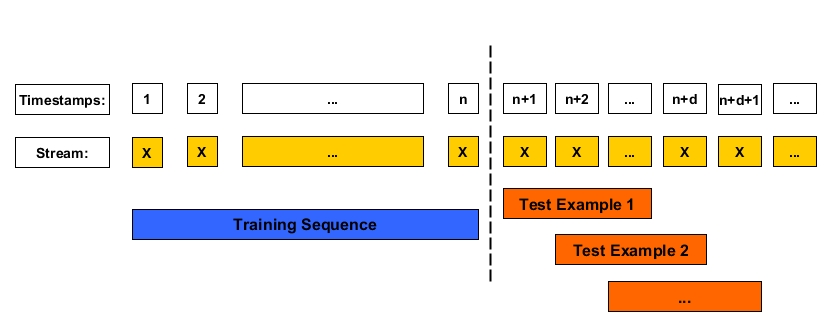
\includegraphics[width=0.75\textwidth]{testData}
	\caption{Test Example Collection for evaluating the models}
	\label{fig_testData}
\end{figure}

\subsection{Rate of Return and Investment Strategies}
\label{subsec_investmentStrageties}
Before we can talk about the rate of return we must first understand simple investments, that can be made at a stock market. There two basic events that are relevant: The stock of a company can rise or fall. For each of these there is an appropriate investment. \\
Let us say an investor predicts a rise in stock value. In this case the investor will buy one of the stocks and then sell it after the price has risen, which leaves the investor with the price difference as a net-gain. In financial jargon this is also called a long investment, or simply long. \\
If however the stock price is expected to fall, it is still possible to make profit by doing the following: First the investor borrows stocks from someone and then immediately sells them for the current price. Then after the price has fallen, the investor buys the stocks for the now lower price and gives them back to the lender. Once again the investor makes profit based on the price difference, assuming the lender does not require the investor to pay a fee. This sort of investment is called a short investment, or simply short. \\
There are a few things to note here:
\begin{itemize}
	\item It is easy to see that if the investor's prediction is incorrect he or she will lose money. The loss is also equal to the difference between current and future stock value.
	\item Shorts usually require an additional fee, that needs to be payed to the lender for borrowing the stocks. However in this evaluation we will assume that such a fee does not exist.
\end{itemize}

Having explained the basic types of investments, it is easy to create an investment strategy based on the model's predictions. This investment strategy is depicted in algorithm \ref{alg_investmentStrategy}. 

\begin{algorithm}[H]
  \caption{Investment Strategy
    \label{alg_investmentStrategy}}
  \begin{algorithmic}[1]
    \Statex
    \Require Let $M$ be the predictive Model, $W$ the current window of the Stream and $t$ the time delay.
    \Function{WindowMining}{}
      	\If{$M(W) = UP$}
      		\State make a long investment, re-sell Stock $t$ seconds later
		\ElsIf{$M(W) = DOWN$}
			\State make a short investment, re-buy Stock $t$ seconds later
       	\EndIf
    \EndFunction
  \end{algorithmic}
\end{algorithm}

It is a very basic strategy that entirely relies on the model output. The only remaining parameter to determine is $t$, the time at which we want to re-sell (in case of longs), or re-buy (in case of shorts) the stocks. Recall that in the training process of the models, we select our examples, by cutting off the window just before the target event, meaning we train the model to recognize situations, in which the next incoming event is the target event. Thus in the general case $t$ should be set to the expected time difference between two timestamps in the stream. Of course, not all streams have a constant update rate in which case things get more complicated. For this specific dataset however, we know that the stream is sampled at a 15 second interval, which is why we set $t = 15s$. \\
After having defined how investments are made, we can finally define the rate of return for an investment. Given the $S$ as the amount of money that was invested, and $E$ as the amount of money left after the investment the rate of return is defined as $r = \frac{E-S}{S}$. As models are being evaluated as described in the previous subsection, many investments will be made, which is why we can define the total rate of return for a model as the sum of all the individual returns that are obtained during the model evaluation.\\
There are a few assumptions, that we need to make in order for this to work. these are:

\begin{itemize}
	\item Short or long investments can be made at any time and they can be made instantaneously.
	\item Making these investments has no influence on the stock price.
	\item Making these investments has no additional cost.
\end{itemize}

Depending on the scenario these assumptions can be more or less realistic and it is important to keep that in mind when looking at the model's rate of return. They will probably not translate one to one to the real world. Apart from that, the rate of return is representing the ground truth about a model, given that the underlying data is valid. The higher the rate of return, the better is the model. Additionally, the rate of return is the metric that users of these models would be most interested in.

\subsection{Accuracy}
The way that the prediction of the stock movement is tackled in this thesis is essentially a three-class classification problem. The value of a stock can either rise, fall or remain equal. It is also clear, that for all test examples, we know the actual class, which means that we can record all test results in a confusion matrix, as shown in figure \ref{fig_confusionMatrix}.
\\
\begin{figure}[h]
\centering
\begin{tikzpicture}[
box/.style={draw,rectangle,minimum size=2cm,text width=1.5cm,align=left}]
\matrix (conmat) [row sep=.1cm,column sep=.1cm] {

\node (tpos) [box,
    label=left:\( \mathbf{UP} \),
    label=above:\( \mathbf{UP} \)
    ] {$U_{U}$};
&
\node (fneg) [box,
    label=above:\textbf{EQUAL}] {$U_{E}$};
&
\node (fneg2) [box,
    label=above:\textbf{DOWN}] {$U_{D}$};
\\


\node (fneg3) [box,
    label=left:\textbf{DOWN}] {$E_{U}$};
&
\node (tpos2) [box] {$E_{E}$};
&
\node (fneg4) [box] {$E_{D}$};
\\

\node (fneg5) [box,
    label=left:\textbf{DOWN}] {$D_{U}$};
&
\node (fneg6) [box] {$D_{E}$};
&
\node (tpos3) [box] {$D_{D}$};

\\
};
\node [left=.05cm of conmat,text width=1.5cm,align=right] {\textbf{actual \\ value}};
\node [above=.05cm of conmat] {\textbf{prediction outcome}};
\end{tikzpicture}
\label{fig_confusionMatrix}
\caption{Confusion Matrix example}
\end{figure}

The classical evaluation metric of classifier accuracy would be calculated by summing the diagonal from top-left to bottom-right and dividing by the sum of all matrix entries. However, with the way that the automatic investments work, this is counter intuitive, since we are penalizing the classifier for actions that are not necessarily hurtful. The obvious case is the misclassification of UP or DOWN events as EQUAL. Since no actions are taken, this does not have a negative impact overall. It can be seen as a lost opportunity, but it is not nearly as hurtful as mistaking UP for DOWN, so counting both equally is undesirable. Also the other case, in which an EQUAL event gets incorrectly classified as an UP or DOWN event is not hurtful, at least given the assumptions about investments made in subsection \ref{subsec_investmentStrageties}. This means that in the evaluation of this setting, it is useful to discard the EQUAL events and misclassifications. This essentially turns the setting into binary classification, where accuracy is defined as:

\[ Acc = \frac{U_U + D_D}{U_U +U_D +D_U+D_D}\]

Therefore whenever we mention accuracy in the evaluation the formula above is meant. There are other evaluation metrics that could be considered, such as Precision, Recall or Area under ROC-curve. These will not be used in this evaluation, since all the test samples have a rather well-balanced class distribution.



\section{Evaluation Result}
\label{sec_evaluationResults}

\subsection{Explorative Analysis}
\label{subsec_explorativeAnalysis}

As a first exploratory analysis the following configuration was selected for the algorithms:

\begin{itemize}
	\item $d = 90s$
	\item $m = 100$ 
	\item $s_P = 0.8$
	\item $s_S = 0.8$
	\item $n = 20$ (only relevant for PERMS)
\end{itemize}

A Model was trained for each approach and for each company, resulting in 80 different models, using this configuration. Figure \ref{fig_firstRunReturnByCompany} shows the rate of return for each model.

\begin{figure}[h]
	\centering
  	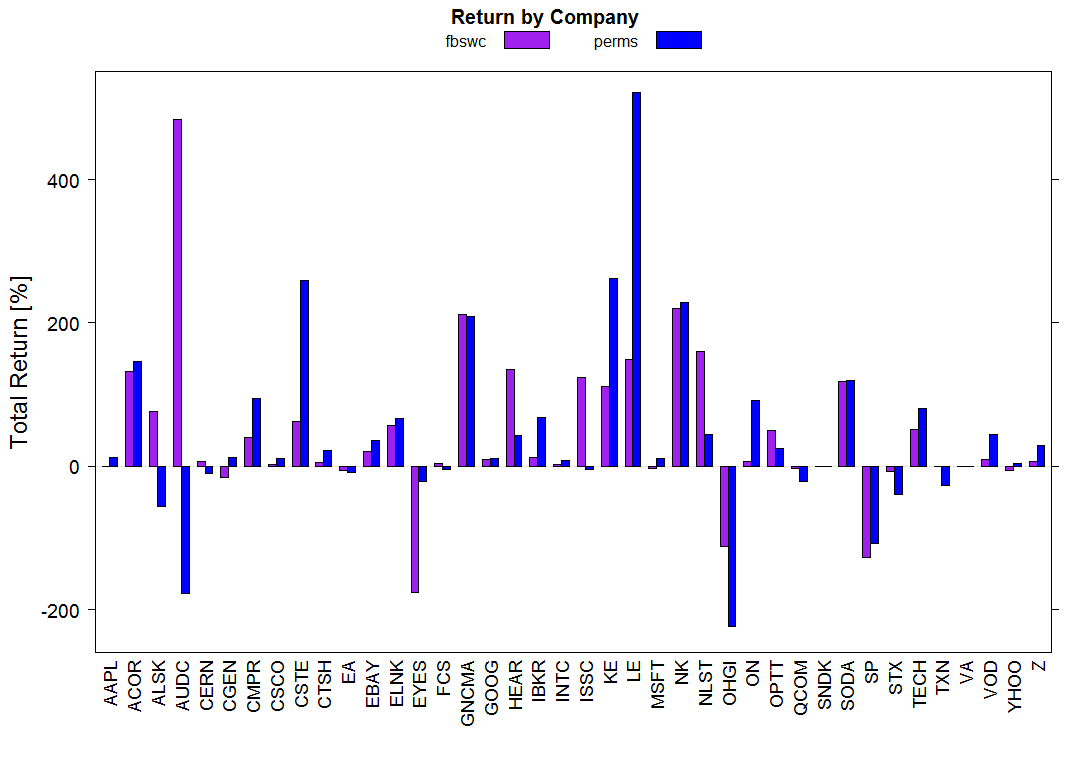
\includegraphics[width=0.75\textwidth]{firstRunReturnByCompany}
	\caption{Histogram: Rate of Return}
	\label{fig_firstRunReturnByCompany}
\end{figure}

The histograms shows that there is quite a large disparity between the different models for the different companies. Table \ref{table_firstRunReturn} shows the average return values over the models, as well as the standard deviation.

\begin{table}
\label{table_firstRunReturn}	
\caption{Mean and STD of the model's Return}
\begin{tabular}{ c | c | c }		
  Model Type & mean(Return)  $[\%]$ & std(Return) $[\%]$ \\
  \hline
  PERMS & 44.0 & 124.3 \\
  FBSWC & 45.4 & 107.3 \\
\end{tabular}
\end{table}

 The first thing to note here is that the mean values of 0.44 and 0.45 for return are extremely high. This essentially means that on average, automatic trading algorithms using the models built by the methods suggested in this paper would make a profit of $44\%$ or $45\%$ respectively. These would be amazing results in a real-life scenario. However there are a few things to be noted here. First of all, the standard deviation is higher than the actual mean in all cases, meaning there is a large variance in model performance. A look at the boxplots in figure \ref{fig_returnBoxplots} confirms this.
 
\begin{figure}[h]
\centering
\begin{subfigure}{.5\textwidth}
  \centering
  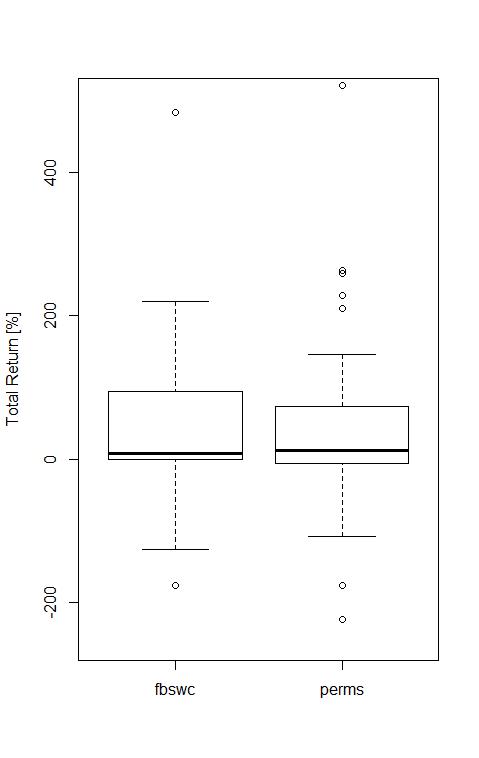
\includegraphics[width=\linewidth]{boxplotReturn}
  \label{fig_returnBoxplot}
  \caption{Return}
\end{subfigure}%
\begin{subfigure}{.5\textwidth}
  \centering
  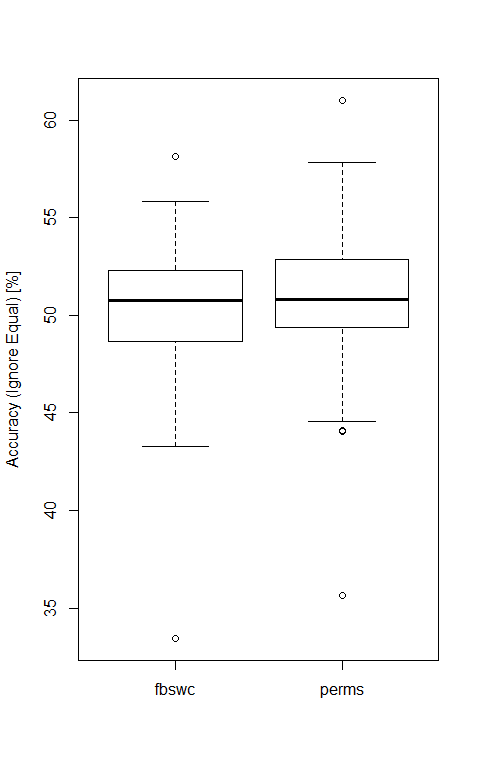
\includegraphics[width=\linewidth]{boxplotAccuracy}
  \label{fig_accuracyBoxplot}
  \caption{Accuracy}
\end{subfigure}
\caption{Boxplots for Return and Accuracy, grouped by Model Type}
\label{fig_returnBoxplots}
\end{figure}

These plots seem to suggest that the algorithms produce models with a high range of quality, either being outstanding like the FBSWC-model for the stock of \textit{AUDC} or extremely weak, like the PERMS-model for the stock of \textit{OHGI}. This seems rather weird, but could be explained by some stocks being easier to predict than others. However, when looking closer at the classical evaluation metrics for classification, it becomes clear, that something is amiss. Figure \ref{fig_accuracyByCompany} plots the accuracy values (ignoring equal events and misclassifications as equal as described in TODO) for the different models. 

\begin{figure}[h]
	\centering
  	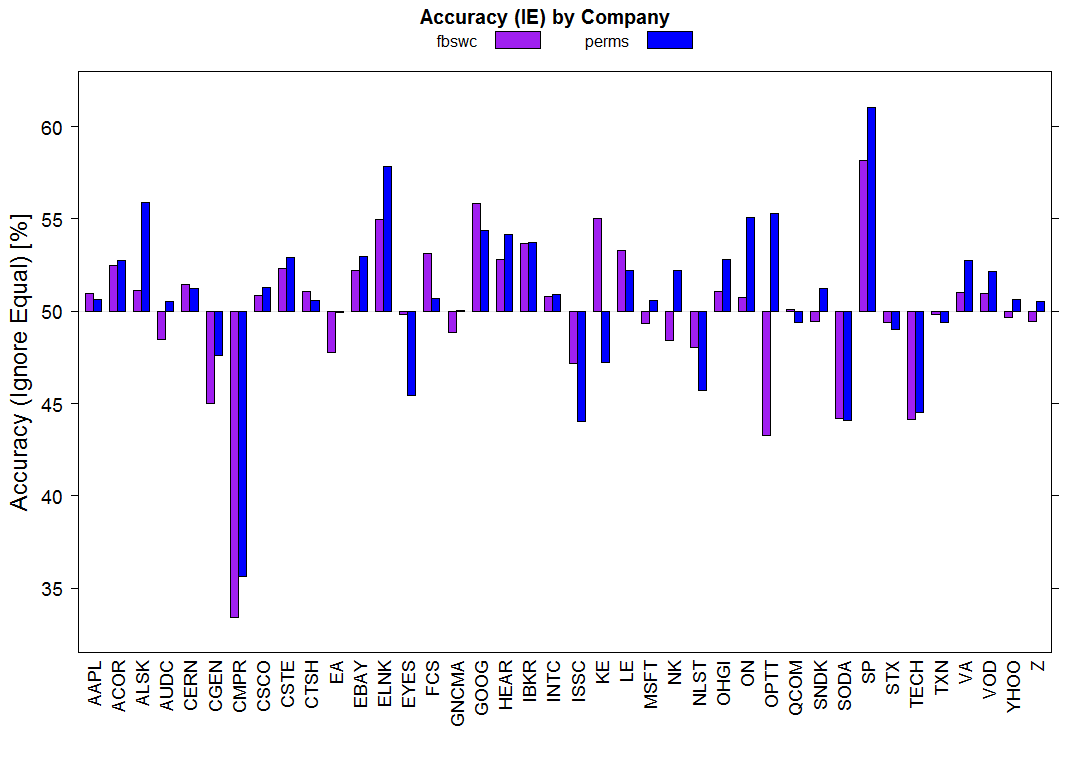
\includegraphics[width=0.75\textwidth]{accuracyByCompany}
	\caption{Histogram: Accuracy (Ignore Equal)}
	\label{fig_accuracyByCompany}
\end{figure}

The origin of the x-axis is set to $50\%$ accuracy, since this is essentially the border we want to overcome. A model with above $50\%$ accuracy is expected to make profits, a model below $50\%$ accuracy is expected to make losses. At first the plot seems to be somewhat consistent with earlier observations, since a majority of models is above $50\%$ accuracy. However, when taking a closer look, it becomes clear that these two metrics contradict each other. Consider the stocks of \textit{CMPR} for example. The accuracy values for both models are extremely poor, however both models apparently net profits, as shown in figure \ref{fig_firstRunReturnByCompany}. One quickly notices similarly weird examples, like the model for the stock \textit{SP}, which performs well accuracy-wise, but nets losses, as shown in the return metric. Additionally the accuracy distibution as shown in table \ref{table_firstRunAccuracy} and boxplot \ref{fig_accuracyBoxplot} has a rather low variance, compared to the return metric.

\begin{table}
\label{table_firstRunAccuracy}	
\caption{Mean and Standard Deviation of the model's Accuracy}
\begin{tabular}{ c | c | c}		
  Model Type & mean(Accuracy) $[\%]$ & std(Accuracy) $[\%]$\\
  \hline
  PERMS & 50,7 & 4,3\\
  FBSWC & 50,0 & 4,1\\
\end{tabular}
\end{table}

 So if the accuracy varies very little, how is it possible that the rate of return is so different for many models? Furthermore, the mean accuracy is actually only slightly above $50\%$ for PERMS and exactly $50\%$ for FBSWC. This can simply not explain an average return of $44\%$ or $45\%$? This discrepancy brings a useful thought to mind: What return would we actually expect the model to have, based on its performance recorded in the confusion matrix? \\

\subsection{Expected Return and Deviation Analysis}
Given the confusion matrix of a model and the time series of the corresponding stock value, we can easily estimate what return we would expect from the automatic investment algorithm explained in subsection \ref{subsec_investmentStrageties}. Let
\begin{itemize}
	\item $TP$ be the number of true positives, (Up correctly classified as UP)
	\item $FP$ be the number of false positives (DOWN incorrectly classified as UP)
	\item $FN$ be the number of false negatives (UP incorrectly classified as DOWN)
	\item $TN$ be the number of true negatives (DOWN correctly classified as DOWN)
\end{itemize}
% $TP$ be the number of true positives, (Up correctly classified as UP), $FP$ be the number of false positives (DOWN incorrectly classified as UP), $FN$ be the number of false negatives (UP incorrectly classified as DOWN) and $TN$ be the number of true negatives (DOWN correctly classified as DOWN).
Furthermore let $TS = [v_1,...v_n]$ be the time series of stock values. We define $D = [d_1,...,d_{n-1}]$, where $d_i = \frac{v_{i+1} - v_i}{v_i}$ as the relative difference vector of $TS$. Furthermore let $D^+ = [v1,...v_m]$, where $v_i \in D \land v_i > 0$ and let $D^- = [w1,...w_o]$, where $w_i \in D \land w_i < 0$.  Then we can define the average relative increase as \[INC  = \frac{\sum_{d \in D^+} d}{|D^+|} \] and the average relative decrease as \[ DEC = |\frac{\sum_{\substack{d \in D^-}} d}{|D^-|}| \]
With that we can define the expected return as \[ER  = TP \cdot INC + TN \cdot DEC - FP \cdot DEC - FN \cdot INC \]
If there are no significant outliers or an especially high variance in the multisets $D^+$ and $D^-$ we would expect the return of the automated investment strategy model to behave according to the formula above. With this in mind we simply created a random guessing model for each stock, calculated the actual return as well as the expected return for each model and sorted them according to the absolute difference between these two values. The result is shown in figure \ref{fig_returnDiscrepancy}.

\begin{figure}[h]
	\centering
  	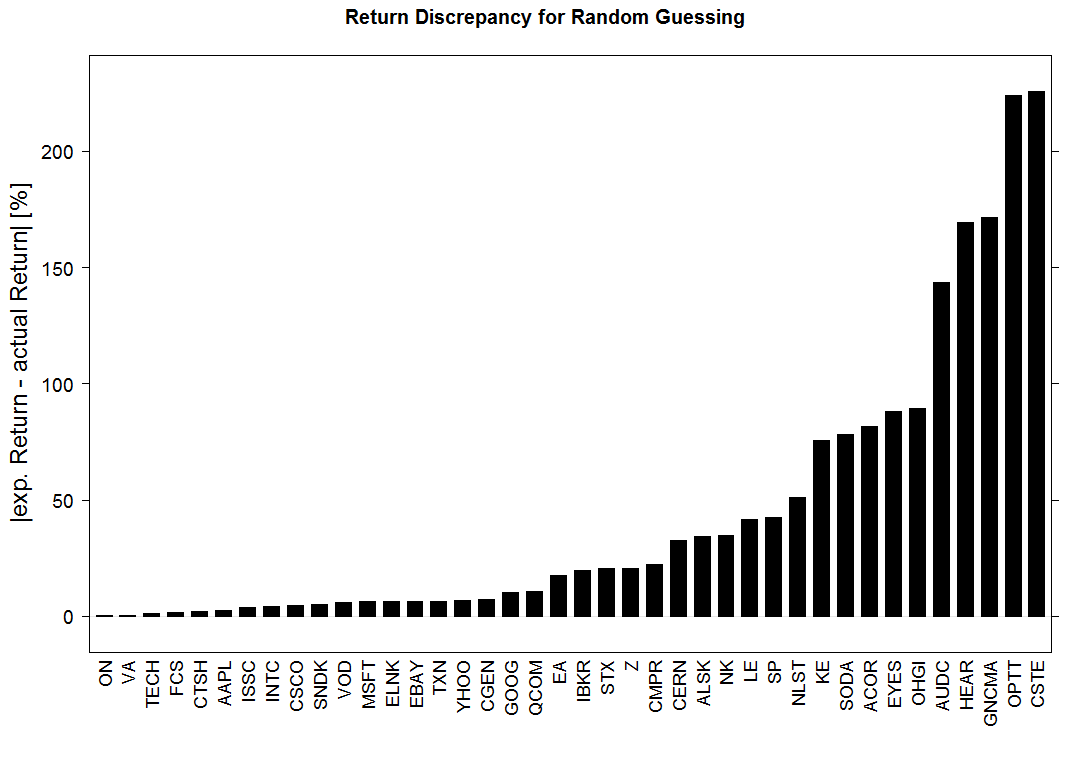
\includegraphics[width=0.75\textwidth]{returnDiscrepancy}
	\caption{Discrepancy between expected and actual return for each model}
	\label{fig_returnDiscrepancy}
\end{figure}

Note that the companies are now no longer ordered alphabetically, but according to the discrepancy of their predictive models. We can see that this discrepancy is quite high for some models. We have now found out that there is not only a discrepancy between the accuracy and return metric of the actual models analyzed in the previous subsection but also for a completely new type of model (the random-guessing model). This strongly suggests that there was no mistake in the model evaluation in the previous section but that instead the problem lies within the underlying data, since a completely new model shows similar discrepancies. The most likely causes for this are high variances or extreme outliers in $D$. Further investigation shows that there is indeed some correlation between the discrepancy and the variance in $D$. Figure \ref{fig_stdDiscrepancy} visualizes this.

\begin{figure}[h]
	\centering
  	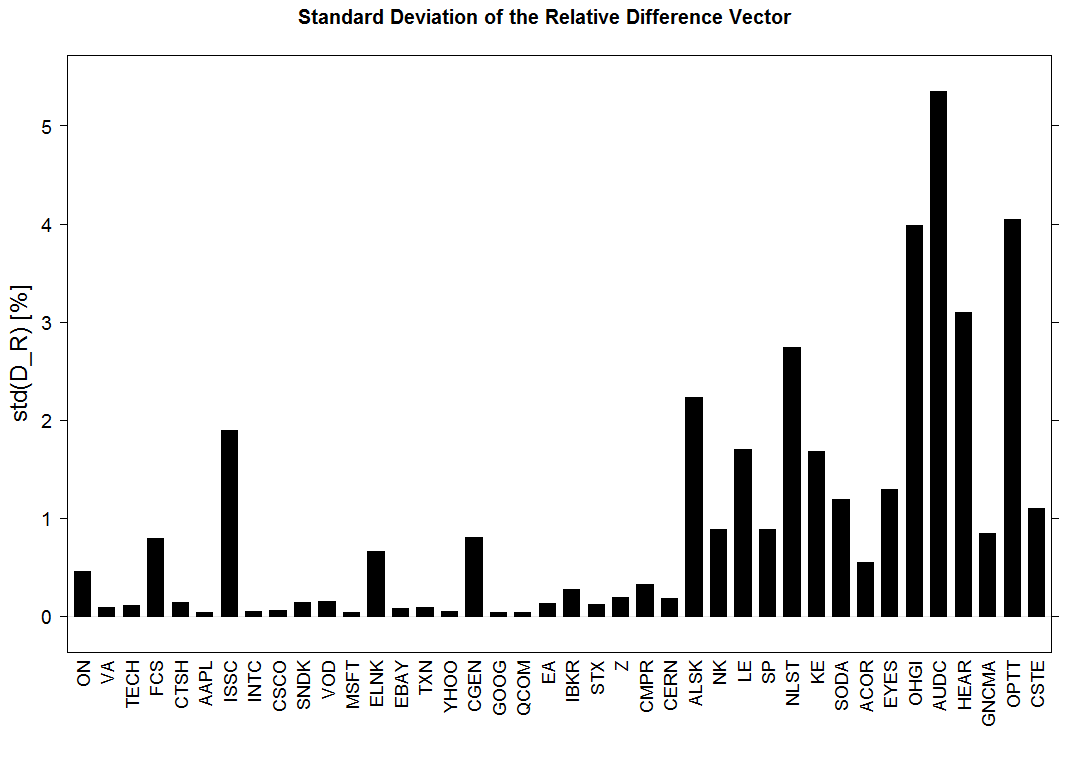
\includegraphics[width=0.75\textwidth]{stdDiscrepancy}
	\caption{Standard Deviation of the relative Difference Vector. Companies have the same order as in figure \ref{fig_returnDiscrepancy}}.
	\label{fig_stdDiscrepancy}
\end{figure}

It can be seen that most of the models with a high discrepancy have a rather high standard deviation in the relative difference vector. There are however notable exceptions, so this is not fully conclusive. An exemplary study of the distribution of the relative difference vector for the company \textit{ACOR}, which has a rather high discrepancy but comparably low standard deviation still reveals that outliers are a probable cause for the high discrepancy. Figure \ref{fig_acorDRDistribution} plots the distribution of \textit{ACOR's} relative difference vector in a boxplot.

\begin{figure}[h]
	\centering
  	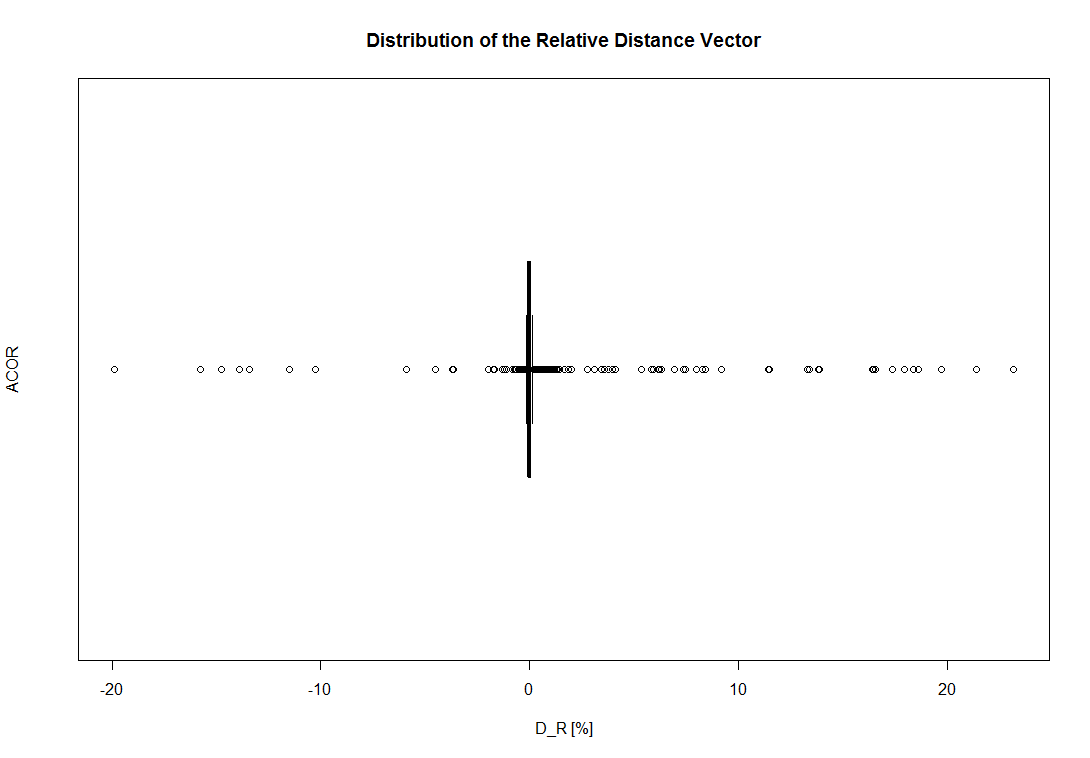
\includegraphics[width=0.75\textwidth]{acorDRDistribution}
	\caption{Distribution of the relative difference vector for company \textit{Acor}. The Distribution contains 24175 values in total. All that can be seen in the figure are outliers according to the definition of a boxplot, since the great majority of the values are inside the box, which is only visible as a horizontal line around 0\%}.
	\label{fig_acorDRDistribution}
\end{figure}

The boxplot shows that it is in fact not unlikely to achieve a high discrepancy between expected (based on the mean difference) and actual return. In order to reach \textit{Acor's} discrepancy of about $80\%$ it is sufficient to get the predictions for the top 4 largest values of $|D|$ wrong, since they have a value of around $20\%$ each. If the remaining predictions are evenly distributed the result will be around $80\%$ higher or lower than expected. \\
This analysis has shown us several things. It has confirmed that many of the financial time series we used as a data basis are at times volatile, which can be a problem for model evaluation. Interestingly, when looking back at the mean results of the models in table \ref{table_firstRunReturn} it seems to be the case that the models get the extreme cases right more often than they get them wrong, since their performance in terms of return is higher than expected instead of lower. Since there were only 40 models evaluated however, this may well be due to chance. \\
It is clear that these extreme outliers in most of the time series are something that models in a real-life scenario must absolutely consider and even be built for to recognize, since misidentifying them would lead to significant losses of money. However these outliers make it hard to asses the quality of the underlying algorithms, which is what we aim to do in this evaluation. This means that from now we will restrict ourselves to the accuracy measure to judge the quality of models (and by proxy the quality of the algorithms).

\subsection{Comparison with Baselines}
As presented in section TODO the state of the art forecasting models for financial time series are rather elaborate and require careful training. Additionally most of the state of the art models forecast daily closing values and thus would need to be modified to fit into the streaming environment. This would require considerable time which is why we do not directly compare our approaches to the state of the art. However since it is necessary to put the performance of the algorithms PERMS and FBSWC in some sort of context, we will compare them to a simple baseline. A very simple forecasting method is the simple moving average method \cite{makridakis1982accuracy} in which a value of the timeseries $v_t$ is forecasted to be the average of the recent values:

\[v_t = \frac{\sum_{i=1}^d v_{t-i}}{d}\] 

This simple baseline can be adapted easily to output categorical predictions like the other predictive models: If the forecasted value for $v_t$ is higher than $v_{t-1}$ we expected the stock to rise, if it is lower we expect the stock to fall and if it is equal we expect the value to remain equal. This is a rather useful baseline, since it this algorithm produces very simple models of which it is reasonable to expect that they are worse than the state of the art. Thus PERMS and FBSWC must do better than this baseline at least if they want to have a chance to compete against the state of the art models. Unfortunately that is not the case. As figure \ref{fig_baselineComparisonBarchart} shows PERMS and FBSWC do not consistently beat the simple moving average model, in fact the simple moving average model scores very high accuracy for a few models and performs worse only a couple of times.

\begin{figure}[h]
	\centering
  	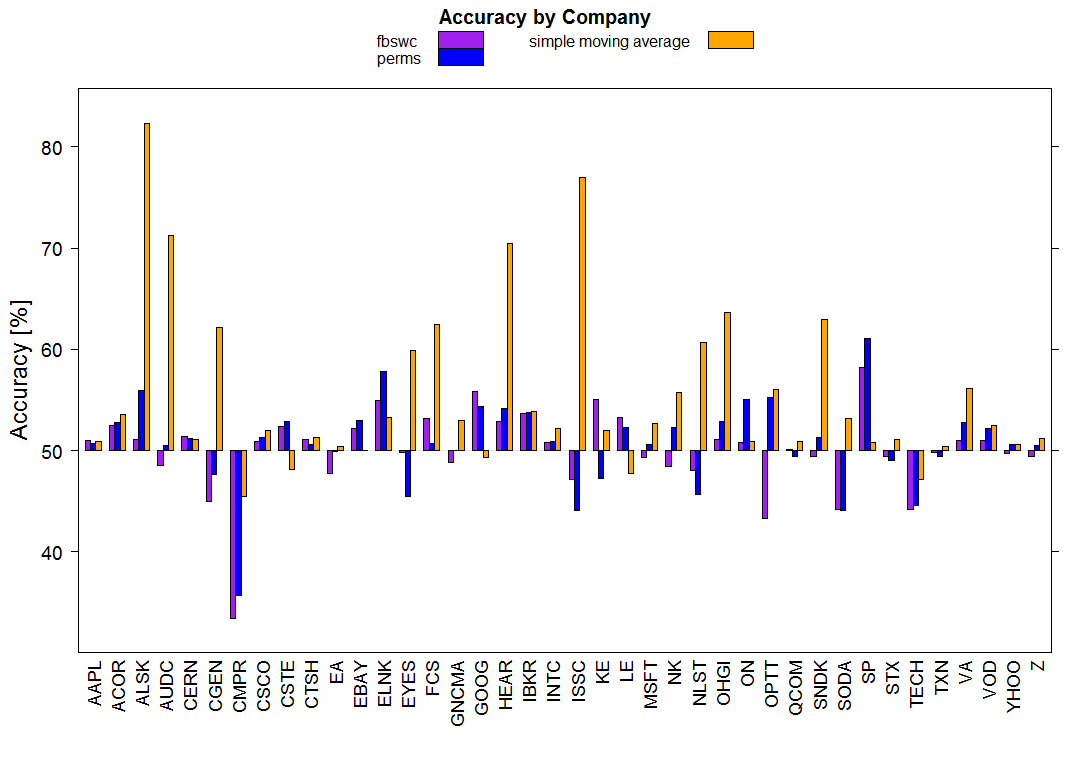
\includegraphics[width=0.75\textwidth]{baselineComparisonBarchart}
	\caption{Comparison of PERMS and FBSWC to the simple moving average baseline in terms of accuracy}
	\label{fig_baselineComparisonBarchart}
\end{figure}

This also shows in the aggregated statistics shown in table \ref{table_baselineAccuracy}. 

\begin{table}
\label{table_baselineAccuracy}	
\caption{Mean and Standard Deviation of the model's Accuracy}
\begin{tabular}{ c | c | c}		
  Model Type & mean(Accuracy) $[\%]$ & std(Accuracy) $[\%]$\\
  \hline
  PERMS & 50.7 & 4.3\\
  FBSWC & 50.0 & 4.1\\
  Simple Moving Average & 55.4 & 8.1\\
\end{tabular}
\end{table}

With a mean accuracy of $55.4\%$ the simple moving average outclasses both the PERMS and FBSWC algorithms in terms of accuracy. There can be a couple of reasons for that. For instance the parameters for PERMS and FBSWC may be poorly chosen. This possibility is explored in the next subsection, where parameters are modified. Additionally, it is important to keep in mind that both PERMS and FBSWC were designed to predict events in categorical streams. Predictions in financial time series, which are numerical streams, may not be the best application domain for these algorithms, since the transformation to categorical data leads to a loss of information, that the simple moving average model does not suffer from. On top of that the simple moving average considers the most recent, and only the most recent data. PERMS and FBSWC are trained at the beginning of the stream and then continuously applied to the stream. Since the models are not yet evolved with the stream it is possible that they learn rules, which become outdated quickly, which in turn hurts their performance.


\subsection{Algorithm Parameter Influence}
Recall that subsection \ref{subsec_explorativeAnalysis} introduced an initial configuration for the algorithms. We refer to this as the base configuration which is now modified. The first parameter to modify is the support for the serial episodes, which can be lowered to allow for a more exhaustive search for predictive patterns. Figure \ref{fig_supportBoxplots} visualizes the accuracy distribution for PERMS and FBSWC for different serial support thresholds as boxplots.

\begin{figure}[h]
\centering
\begin{subfigure}{.5\textwidth}
  \centering
  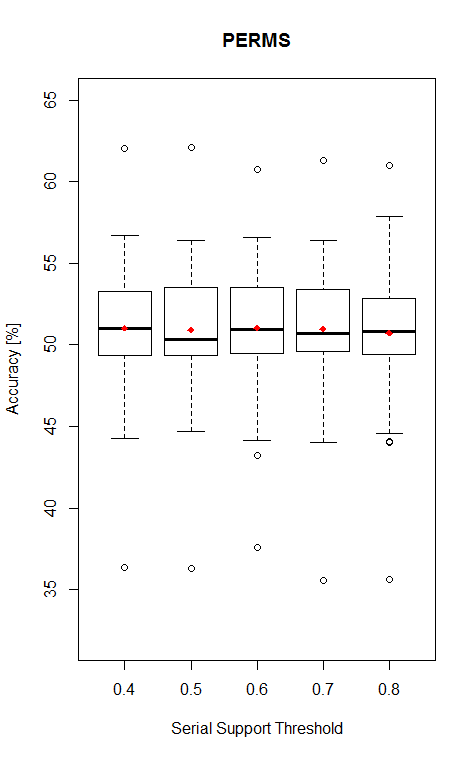
\includegraphics[width=\linewidth]{permsSupportSerial}
  \label{fig_permsSupportSerial}
  \caption{PERMS}
\end{subfigure}%
\begin{subfigure}{.5\textwidth}
  \centering
  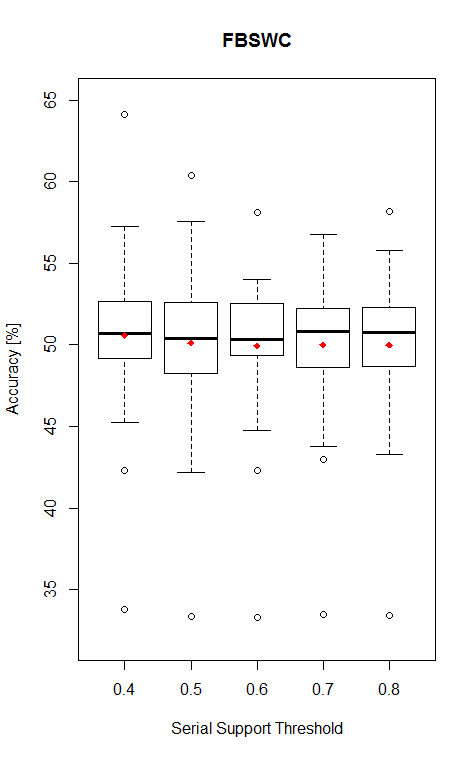
\includegraphics[width=\linewidth]{fbswcSupportSerial}
  \label{fig_fbswcSupportSerial}
  \caption{FBSWC}
\end{subfigure}
\caption{Accuracy distributions for both model types, grouped by support thresholds. The red dots mark the mean accuracy over all models in that group.}
\label{fig_supportBoxplots}
\end{figure}

The boxplots show that there seems to be a surprisingly small influence of the support on the overall model performance. In theory a smaller support threshold should lead to better models, since more episodes will be mined, which increases the chance of finding good predictors. It is however entirely possible that the episodes that occur often also have the best confidence (in case of PERMS) or their derived features have the best information gain (in case of FBSWC), in which case they would be discovered in all the settings. \\
The next parameter that was modified is the number of training windows. Once again the results are shown in several boxplots in figure \ref{fig_numWindowsBoxplots}

\begin{figure}[h]
\centering
\begin{subfigure}{.5\textwidth}
  \centering
  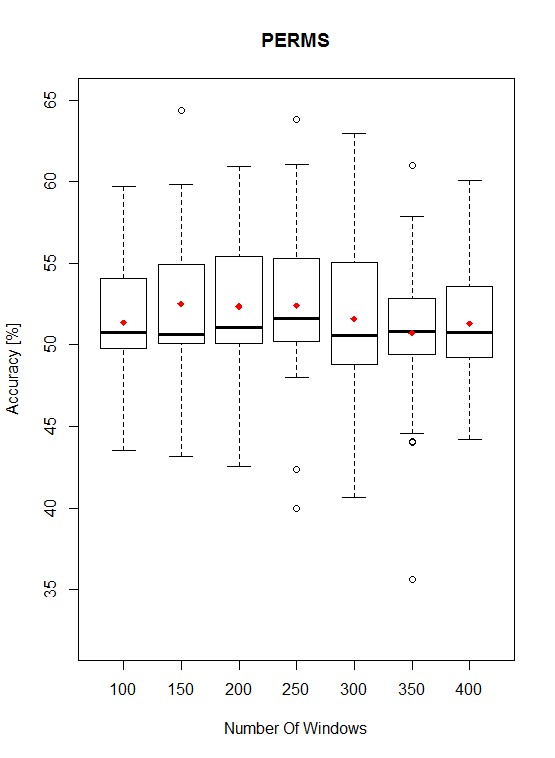
\includegraphics[width=\linewidth]{permsNumWindows}
  \label{fig_permsSupportSerial}
  \caption{PERMS}
\end{subfigure}%
\begin{subfigure}{.5\textwidth}
  \centering
  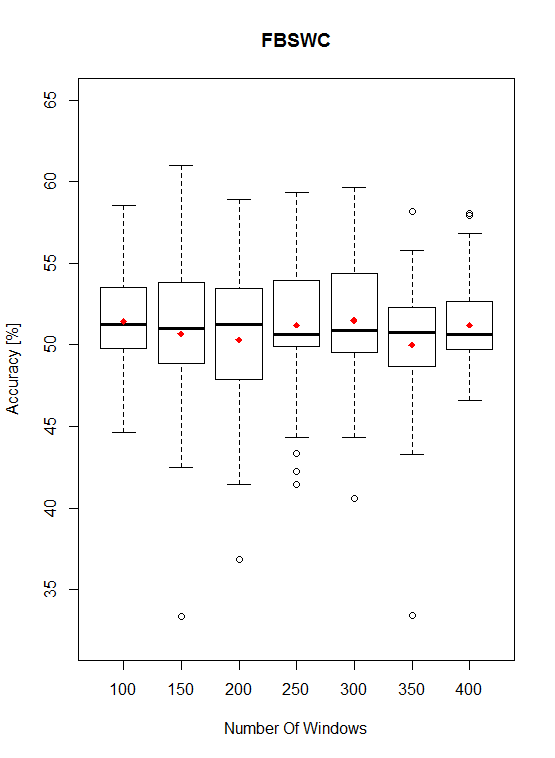
\includegraphics[width=\linewidth]{fbswcNumWindows}
  \label{fig_fbswcSupportSerial}
  \caption{FBSWC}
\end{subfigure}
\caption{Accuracy distributions for both model types, grouped by the number of training windows. The red dots mark the mean accuracy over all models in that group.}
\label{fig_numWindowsBoxplots}
\end{figure}

Overall, the number of training windows seems to have more of an impact than the support threshold for serial episodes, however the impact on model performance is somewhat chaotic. No clear trend can be visibly seen in the boxplots. PERSM does seem to do a littel better with a medium amount of windows (150-250), but the differences are hardly significant. Interestingly the FBSWC-models with the highest number of training examples seem to contain less variance in their performance. However their overall average performance does not increase. \\
The last parameter that was experimented with is the number of predictive episode rules, which is a parameter only for PERMS and somewhat comparable to an ensemble-size parameter. Figure \ref{fig_permsNumPredictors} plots the different accuracy distributions for different numbers of predictive episode rules used in the ensemble.

\begin{figure}[h]
	\centering
  	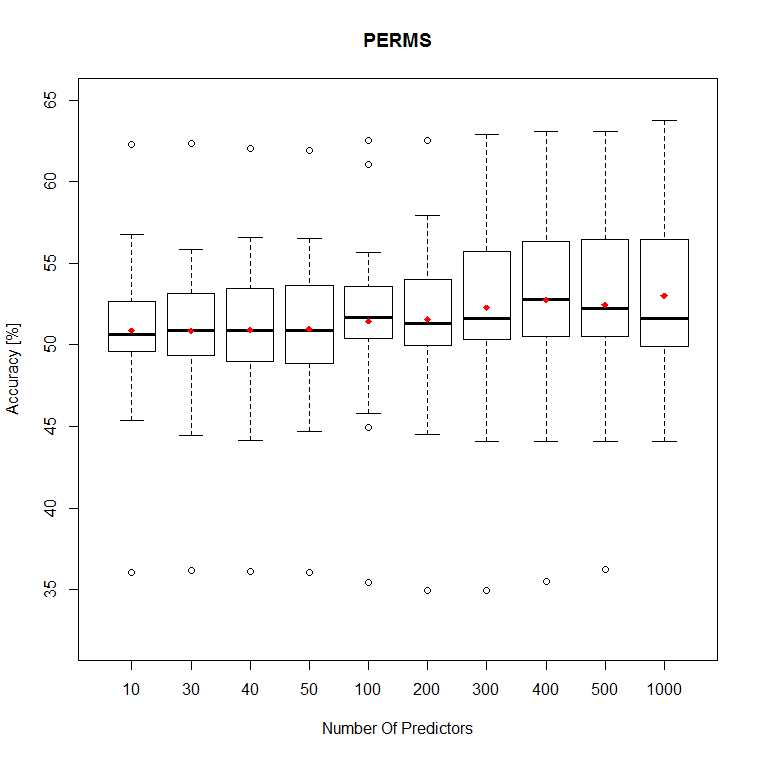
\includegraphics[width=0.75\textwidth]{permsNumPredictors}
	\caption{Accuracy distributions for different ensemble sizes in PERMS. The red dots mark the mean accuracy over all models in that group.}.
	\label{fig_permsNumPredictors}
\end{figure}

In this plot we can finally see an interesting correlation. The mean accuracy over the models increases with rising ensemble-size. This does not eliminate the possibility of failure, since all groups still include poorly performing models, but the general trend seems to go upwards with rising ensemble size. In summary the mean accuracy of the last group (number of predictors set to 1000) is $53\%$, which is an improvement over the $50,7\%$ of the first exploratory run. \\
The window size in seconds was not adjusted in an experimental setting, since window size and support thresholds are closely linked to each other. This due to the fact that larger window sizes will result in more events per window and thus more potential patterns, which means that with rising window size the support thresholds also need to rise to guarantee reasonable runtime and memory requirements of the mining algorithm. \\
In summary, apart from the number of predictive episodes for PERMS there seems to be no significant impact of the tested parameters in this setting. There is also no striking difference between the two learning algorithms PERMS and FBSWC. Models built by both algorithms still tend to score around $50\%$ accuracy, thus they are largely indistinguishable from random guessing. It is interesting however, that both algorithms produce outliers in both directions, which reveals that both algorithms have the potential to build better than random classifiers. The outliers in itself are interesting in that there are some companies whose time series seems to be harder or easier to predict. For example roughly half of the low-accuracy outliers are models built for the time series of company \textit{CMPR}. However the same company also appears in the top-accuracy outliers sometimes, which are overall more diverse.

\subsection{Adding semantics}
As discussed in TODO, the data basis can be enriched by adding and using semantic information about the underlying domain. In our case, we can enrich the datastream by adding derived events using knowledge about the companies. Instead of using the dbpedia \cite{auer2007dbpedia}, we use a simple table provided by the NASDAQ \cite{nasdaqCompanyList}. Among other semantic information, the table assigns each company to an industry sector, which allows us to create derived, aggregated events for each sector. The aggregation process is simple: The underlying numerical streams (of stock values) are grouped by their industry companies and each group is summed to a single value per timestamp. This results in 12 new aggregated streams, which can than be transformed to event streams like described in \ref{subsec_transformation}. The resulting events are new derived events that can be used in the pattern mining stage of the learning algorithms just like regular events. The results using this semantic extension are interesting. First it is important to note, that the support threshold for parallel episodes needed to be increased drastically (from $0.8$ to $0.95$) in order for the mining algorithm to stay within reasonable time and memory bounds. This is due to the fact that it is very unlikely for the aggregated streams to keep the same value over multiple time stamps, which means there will be an event for each aggregated stream at almost every timestamp. This severely worsens the pattern-explosion effect, which can be corrected via very high support values. The remaining parameters were kept the same as in the basic configuration used in the exploratory analysis. The support threshold for serial episodes was modified from $0.6$ to $0.8$ in steps of $0.1$. The mean accuracies are compared in figure \ref{fig_semanticVsNonSemanticAccuracy}. 

\begin{figure}[h]
	\centering
  	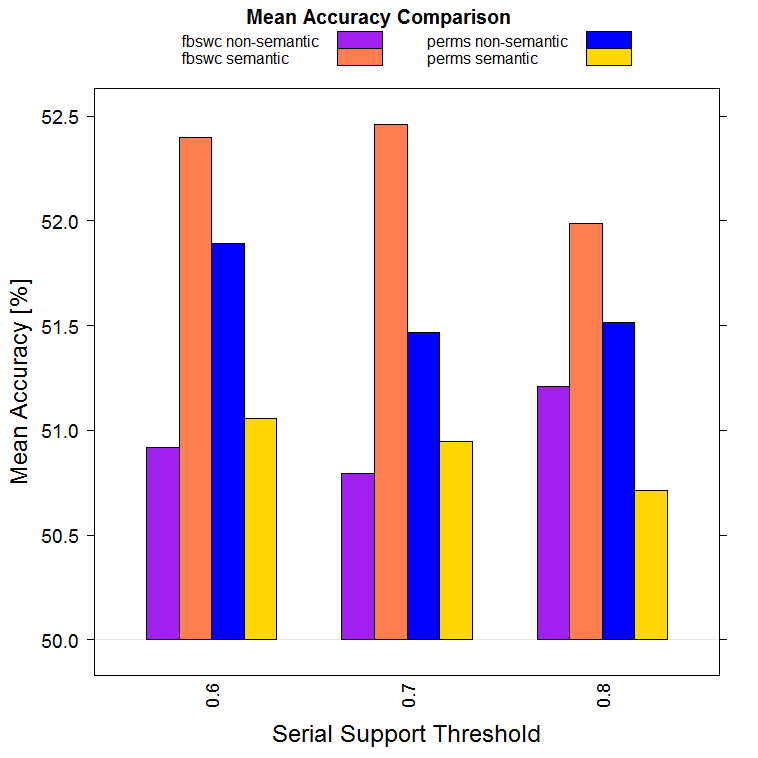
\includegraphics[width=0.75\textwidth]{semanticVsNonSemanticAccuracy}
	\caption{Mean accuracies for different serial support thresholds, grouped by model and whether semantic events were used to enrich the data-stream or not.}.
	\label{fig_semanticVsNonSemanticAccuracy}
\end{figure}

The mean accuracies imply that on average PERMS seems to do a little better without extra semantic knowledge, whereas FBSWC-models seem to profit more from the extra derived events. Figures \ref{fig_permsSupportSerialSemantics} and \ref{fig_fbswcSupportSerialSemantics} take a closer look at the individual accuracy distribution for each model, once with semantically derived events as described above and once without.

\begin{figure}[h]
\centering
\begin{subfigure}{.5\textwidth}
  \centering
  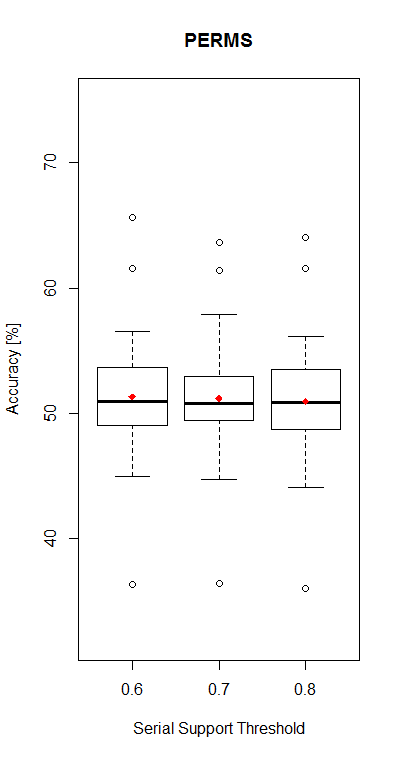
\includegraphics[width=\linewidth]{permsSupportSerialWithSemantic}
  \label{fig_permsSupportSerialWithSemantic}
  \caption{With Derived Events from Semantic Knowledge}
\end{subfigure}%
\begin{subfigure}{.5\textwidth}
  \centering
  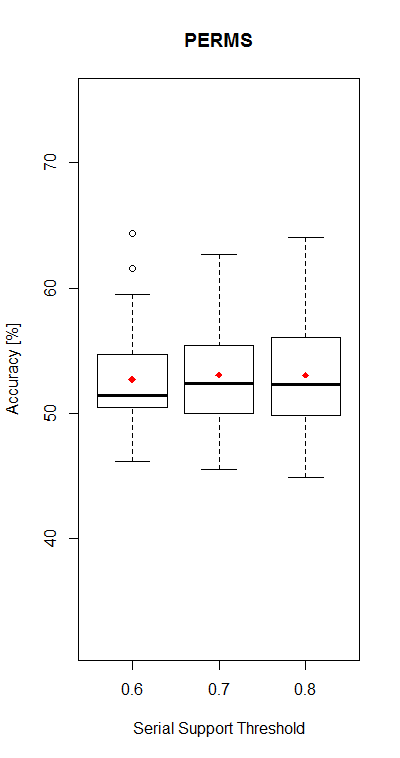
\includegraphics[width=\linewidth]{permsSupportSerialWithOutSemantic}
  \label{fig_permsSupportSerialWithOutSemantic}
  \caption{Without Semantic Knowledge}
\end{subfigure}
\caption{Accuracy distributions for PERMS with different support thresholds for serial episodes, once with semantic enrichment, once without. The red dots mark the mean accuracy over all models in that group.}
\label{fig_permsSupportSerialSemantics}
\end{figure}

\begin{figure}[h]
\centering
\begin{subfigure}{.5\textwidth}
  \centering
  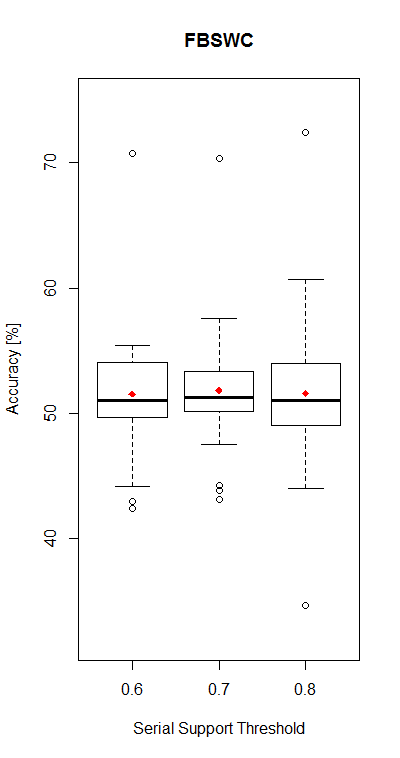
\includegraphics[width=\linewidth]{fbswcSupportSerialWithSemantic}
  \label{fig_fbswcSupportSerialWithSemantic}
  \caption{With Derived Events from Semantic Knowledge}
\end{subfigure}%
\begin{subfigure}{.5\textwidth}
  \centering
  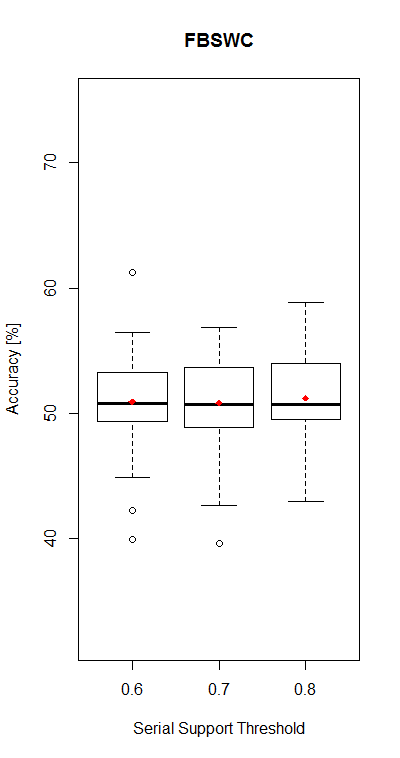
\includegraphics[width=\linewidth]{fbswcSupportSerialWithOutSemantic}
  \label{fig_fbswcSupportSerialWithOutSemantic}
  \caption{Without Semantic Knowledge}
\end{subfigure}
\caption{Accuracy distributions for FBSWC with different support thresholds for serial episodes, once with semantic enrichment, once without. The red dots mark the mean accuracy over all models in that group.}
\label{fig_fbswcSupportSerialSemantics}
\end{figure}

The distributions visualized in these boxplots show that the differences on average are very small, however the outliers imply that there is the potential to build well performing models. This is the first time that any configuration of PERMS or FBSWC was able to build a model with an accuracy of more than $70\%$. This shows that semantic knowledge has great potential to increase predictive performance, even though on average the differences are negligible for this setting. \\
Another possibility is of course to build predictive models for the aggregated event streams themselves and thus predict the movement of industry sectors. The results for this are shown in figure \ref{fig_sectorAnalysis}.

\begin{figure}[h]
\centering
\begin{subfigure}{.5\textwidth}
  \centering
  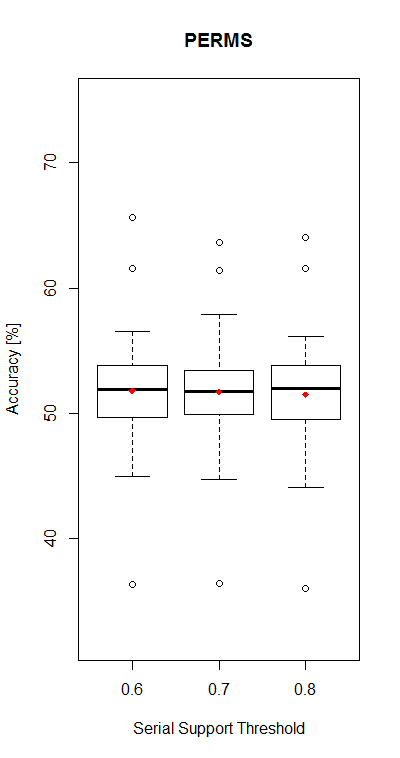
\includegraphics[width=\linewidth]{permsSectorPrediction}
  \label{fig_permsSectorPrediction}
  \caption{Accuracy distribution for PERMS}
\end{subfigure}%
\begin{subfigure}{.5\textwidth}
  \centering
  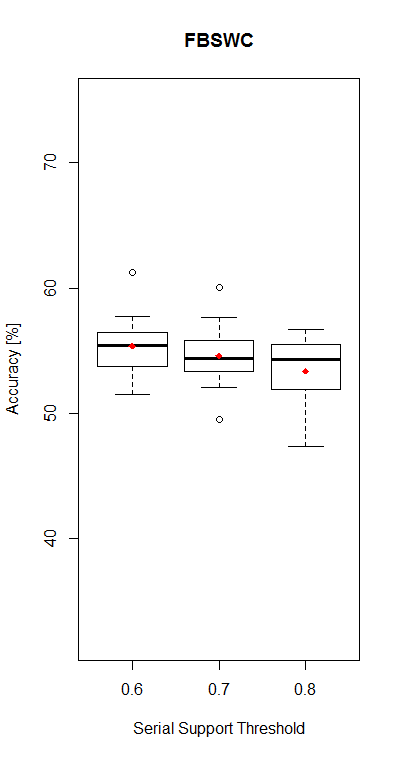
\includegraphics[width=\linewidth]{fbswcSectorPrediction}
  \label{fig_fbswcSectorPrediction}
  \caption{Accuracy distribution for FBSWC}
\end{subfigure}
\caption{Accuracy distributions for the prediction of the aggregated event streams (sector streams), which were added using semantic knowledge.}
\label{fig_sectorAnalysis}
\end{figure}

The results for PERMS are in line with the results for "normal" event streams in previous plots. By contrast, FBSWC with the serial support thresholds $0.6$ and $0.7$ performs better than on the "normal" streams. The models also show lower variance in their accuracy than in previous plots, although one has to keep in mind that in contrast to 40 "normal" models for the companies there are only 12 sector-models.

\subsection{Summary}
In summary the evaluation shows that both PERMS as well as FBSWC have the potential to build well-performing models, however on average the models for the current data-set are largely indistinguishable from random guessing. The different parameters seem to have little impact in this setting with the exception of the ensemble-size for PERMS, where an increasing ensemble-size seems to lead to an increase in performance. Both algorithms show little difference in most parameter settings, however it seems that FBSWC does better with additional semantic information. However predicting up- or downward movements in financial time series seems to be a hard problem for both FBSWC and PERMS as both algorithms struggle to produce models that are better than random guessing, clearly losing out to the baseline approach of simple moving averages. Both algorithms definitely have the potential to be improved though, since as of now they do not utilize the online learning mechanisms as suggested in \ref{sec_EvolvingModels}.